%
% Angepasste FOM Seminarvorlage
%
\documentclass[12pt,a4paper,listof=totoc,bibliography=totoc]{scrartcl}

\usepackage[english]{babel}			% englische Namen/Umlaute
\usepackage[utf8]{inputenc}	    	% Zeichensatzkodierung
\usepackage{fancyhdr}
\usepackage{graphicx}               % Einbinden von Bildern
\usepackage[hidelinks]{hyperref}	% Klickbare Verweise und \autoref{label}
\usepackage[intoc]{nomencl}
\usepackage{setspace}
\usepackage{parskip}
\usepackage{caption}
\usepackage{float}
\usepackage{listings}
\usepackage{geometry}
 \geometry{a4paper, left=40mm, right=20mm, top=40mm, bottom=20mm}
\renewcommand{\familydefault}{\sfdefault}
\renewcommand{\ttdefault}{pcr}
\renewcommand{\lstlistlistingname}{List of Examples}
\renewcommand{\lstlistingname}{Example}

% Bildueberschrift oben und rechtsbuendig
\captionsetup{labelfont=bf, textfont=bf}
\captionsetup{justification=raggedright,singlelinecheck=false}

% Blocksatz
\def\justify{%
  \rightskip=0pt
  \spaceskip=0pt
  \xspaceskip=0pt
  \relax
}

%
%	Hier werden Titel, Bearbeiter und das Datum eingetragen
%
\newcommand\svthema{Web Traffic Analysis - Predicting Blog Post Performance}
\newcommand\svperson{Christian Frank (\#473088)}
\newcommand\svdatum{\today}
\newcommand\lvname{Wirtschaftsinformatik: Big Data \& Data Science}
\newcommand\lvtyp{WS 2020}
\newcommand\lvinst{FOM - Hochschule für Oekonomie \& Management}
\newcommand\lvbetr{Dr. Marcel Graus}

\hypersetup{ % Thema und Author in die Meta-Daten der PDF
  pdftitle={\svthema}, 
  pdfauthor={Christian Frank},
  pdfsubject={Web Traffic Analysis - Predicting Blog Post Performance},
  pdfkeywords={Web, Traffic, Analysis}
}

\begin{document}

% Titel
\title{ \huge\textbf{\svthema} }
\author{ {\svperson} \\ \svdatum }
\date{ \normalsize \centering 
\includegraphics[width=0.3\textwidth]{FOM}\\ {\lvname} \\ {\lvbetr} \\ {\lvinst} \\ {\lvtyp} }

% Seitennummer oben
\pagestyle{fancy}
\fancyhf{}
\fancyhf[ch]{\thepage}
\renewcommand\headrulewidth{0pt}

\maketitle
\thispagestyle{empty} % laesst die Seitennummer auf der Titelseite verschwinden
\pagenumbering{Roman}

\begin{abstract}
In this paper, I'll analyze blog post performance with data taken by Plausible web-site analytics, enhance it with categorization and sentiment analysis, and aim to make predictions on future blog post performance.

\end{abstract}

\vfill
\begin{figure}[h]
    \centering
    
\includegraphics[]{CC-BY}
\end{figure}

This work is licensed under the Creative Commons Attribution 4.0 International License. To view a copy of this license, visit http://creativecommons.org/licenses/by/4.0/ or send a letter to Creative Commons, PO Box 1866, Mountain View, CA 94042, USA.

\cleardoublepage

\tableofcontents			% Inhaltsverzeichnis
\cleardoublepage

\listoffigures				% Abbildungsverzeichnis
\cleardoublepage

\lstlistoflistings			% Codeverzeichnis
\cleardoublepage

%
% Abkuerzungsverzeichnis
%
\makenomenclature
\renewcommand{\nomname}{List of Abbreviations}

\nomenclature{\textbf{CCPA}}{California Consumer Privacy Act}
\nomenclature{\textbf{CTR}}{Click-Through-Rate}
\nomenclature{\textbf{GDPR}}{General Data Protection Regulation}
\nomenclature{\textbf{KPI}}{Key Performance Indicator}
\nomenclature{\textbf{NLP}}{Natural Language Processing}
\nomenclature{\textbf{PECR}}{Privacy and Electronic Communications Regulations}
\nomenclature{\textbf{RSS}}{Really Simple Syndication}
\nomenclature{\textbf{SMM}}{Social Media Marketing}
\nomenclature{\textbf{SQL}}{Structured Query Language}
\nomenclature{\textbf{URL}}{Uniform Resource Locator}
\nomenclature{\textbf{VADER}}{Valence Aware Dictionary and sEntiment Reasoner}

\printnomenclature[1.5in]          % Abkuerzungsverzeichnis
\cleardoublepage

\pagenumbering{arabic}
\setcounter{page}{5}

%
%	Einfuehrung
%

\pagebreak
\section{Web Traffic Analysis}

\onehalfspacing

\subsection{Web Analytics}

In this paper, I will look at the traffic data of my blog, analyze that data, and then lay the foundation to predict a blog post's performance based on its content.

Web analytics is the domain of the big search engines, and Google Analytics and Google AdSense are the market leaders. In all of Social Media and Social Media Marketing, web analytics plays a key role in evaluating a web site's performance and forms the basis of automated advertising placement.

Page views, bounce rate and unique visitors are key metrics to evaluate a web site and the currency that fuels the internet. Every marketeer or web site owner will use these metrics to analyze performance and identify areas for growth; a lot of tools for analysis have become available in the last couple of years, some of them open-source, some closed-source.

Generally speaking, more traffic can potentially lead to more business opportunities. For a commercial web site, it is absolutely mandatory to monitor its web analytics data on a daily basis and act immediately on any anomaly.

However, a blog does not necessarily have commercial interests and might just be an outlet for personal interests or interactions. Why would we want to look at web analytics anyway?

\subsection{Social Media and Loneliness}

In the current COVID-19 pandemic, social distancing is a key element in containing the spread of the virus. Social distancing over a long period of time can increase loneliness and significantly affect people's health negatively, according to a recent study conducted by the American Psychological Association.\footnote{See \textit{Luchetti, M. (2020)}: The trajectory of loneliness in response to COVID-19. \cite{apaLoneliness}}

In the study, the researchers formulate the hypothesizes, that an increase in perceived support from others can offset the feeling of loneliness during the required isolation.

One element to offset the effects of loneliness is increased interaction on social media, in addition to virtual video meetings. Social media interaction includes blogs. The more engaging a blog post is, the more chances are that it can reach people to whom it will be entertaining or otherwise beneficial.

Thus the aim of this analysis is to get an answer for my blog on the question "On which subject should I post to increase my reach?", using visualization and correlation as the primary means, in the hope of increasing its value for others.

\subsection{Gender-neutral Pronouns}

As we move towards a more inclusive and gender-fluid society, it's time to rethink the usage of gendered pronouns in scientific texts. Two well-known professors from UCLA, Abigail C. Saguy, and Juliet A. Williams argue that it makes a lot of sense to use singular they/them instead: "The universal singular they is inclusive of people who identify as male, female or nonbinary."\footnote{\textit{Saguy, A. (2020)}: Why We Should All Use They/Them Pronouns. \cite{pronouns}} Throughout this paper, I'll attempt to follow their suggestion and am inviting my readers to do the same in future papers, and support an inclusive approach through gender-neutral language. Thank you!


%
%	Begrifflichkeiten
%

\pagebreak
\section{Data Sources and Research Methods}

\onehalfspacing

\subsection{The Blog}

The blog is question is my personal \href{https://chfrank.net/wordpress}{web log} that I started a couple of years ago, initially on the now-defunct Google+ platform. It's now on a hosted WordPress instance provided by a local service provider running on a web server farm in Strasbourg. A move from Google+ to Blogger instead of WordPress might have been the easier choice and also allowed for more consistency, however, now there was a clean break between the hosting platforms and the original Google+ data is lost.

I use the blog to complement my other social media whenever I feel the need to express myself in slightly longer texts. I try to post at least once per week and cross-post the blog entries to my other channels, private as well as professional; for small essays I use Medium to publish.

Although I do cross-post, I never duplicate entries and thus there is no dilution of data; the data from every post is be unique and all content is only published once.

During the current and past COVID-19 lockdowns I wrote a running week-by-week commentary, which does affect the traffic analysis outcome, as we'll see later.

\subsection{Plausible}

The data I'll be using was collected using GDPR-compliant web analytics by Plausible, a lightweight and open-source website analytics tool. Plausible provides an easy-to-use web hook to integrate its analytics with almost any kind of website framework; it is ad-free and offered as Software-as-a-Service with a subscription model.

Plausible does not use any kind of tracking cookies and claims to be fully compliant with GDPR, CCPA and PECR. In addition to the web analytics data, I will complement Plausible's data with additional data taken from the blog itself.

\begin{figure}[H]
\centering
\caption {Plausible Summary}
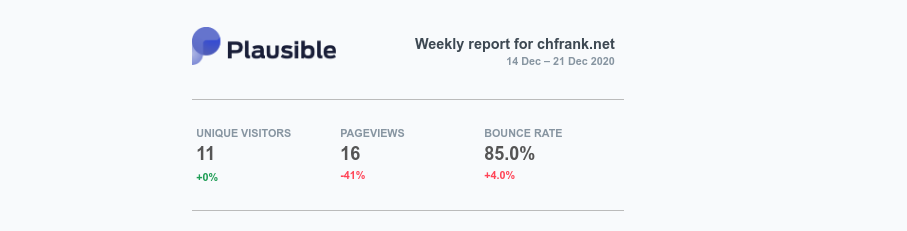
\includegraphics[width=\linewidth]{images/plausible.png}
\label{fig:plausibleSummary}
\end{figure}

In a previous paper, I have covered Plausible in more detail and compared it with other web analytics tools\footnote{See \textit{Frank, C. (2020)}: Usefulness of open-source tools for web analytics in EMarketing .\cite{previousPaper}}; I will not go any further into details of the tool itself in this paper.

In case you're interested, you can find up-to-date raw web traffic data from the blog here: \href{https://plausible.io/chfrank.net}{Plausible Analytics}.

\subsection{Web Traffic KPIs}

In marketing categories, a blog belongs to the realm of inbound marketing, as it tries to offer interesting content and create value for the visitors, but does not reach out by itself. 

Unlike outbound EMail campaigns, for example, that ask the visitor to view a certain website, a blog relies on its content and the willingness of the visitor to actively choose the site for a visit, for example by being pointed to a post from Google search result or a tweet.

In WordPress there is an option to subscribe to a blog to get notification on new posts; WordPress also provides the ability to subscribe to a blog's RSS feed.

In a recent paper on inbound marketing, Yvonne Romes identifies a couple of important KPIs for inbound marketing, a couple of which I will summarize here based on her paper:\footnote{See \textit{Romes, Y. (2020)}: 10 Inbound KPIs, die jetzt auch Personaler kennen sollten .\cite{inboundKPI}}

\begin{itemize}
\item Page Views
\item Bounce Rate
\item Visit Duration
\item Unique Visitors
\end{itemize}

Page Views is the amount of clicks a certain page has received; on a blog usually more page views indicate more engaging content.

Bounce Rate describes the rate of users that leave the site without selecting another links; a high bounce rate can indicate a lack of engaging or interesting content.

Visit Duration is the amount of time a unique visitor spends on the web site; for a blog which mainly offers content to read, a longer duration most likely indicates higher engagement.

Unique visitor is a visitor that can be differentiated from another visitor. Unlike many other platforms, Plausible does not use tracking cookies to identify unique visitors but relies on publicly available information, such as an IP address, to differentiate them. Even though the metric is less accurate with Plausible than with other platforms, it's still an important metric and as before, on a blog more visitors usually indicate higher engagement.

In this paper, these are the four metrics that I will focus on.

\subsection{Statistical Methods}

I will base the analysis on the excellent work and plentiful documentation available at Towards Data Science, a platform on Medium to exchange ideas and to expand the understanding of data science.\footnote{See \textit{TDS Editors (2018)}: About Towards Data Science .\cite{aboutTDS}}

Key elements in data science are statistics and linear algebra.

"From an academic perspective, understanding linear algebra is paramount to having a strong knowledge of specific topics within computer vision and deep learning."\footnote{\textit{Alake, R. (2020)}: 6 Questions Asked By Machine Learning Enthusiasts .\cite{sixQuestions}}

A great reference for using linear algebra in data science and machine learning is the book, "Mathematics for Machine Learning" by Marc Peter Deisenroth, A. Aldo Faisal, and Cheng Soon Ong.\footnote{See \textit{Deisenroth, M.P. (2020)}: Mathematics for Machine Learning .\cite{mathematicsML}}

In this paper I will stay relatively simple and only look at two-dimensional data to identify possible correlations between measurements. I am acutely aware of the fact that "correlation does not imply causation"\footnote{See \textit{Singh, S. (2020)}: Why correlation does not imply causation .\cite{correlateCause}} and will make sure that our findings match real-world scenarios and experiences.

For statistics, I will look at the arithmetic mean, median and mode of our data.

The actual data-set is small, as the blog does not have a lot of traffic, so any method that relies on a high number of data points will not work. For the analysis and predictions of future performance I will rely mainly on visualization techniques and verbal interpretation of the data.

\subsection{Sentiment Analysis}

The blog already has categories for its content, so there's no need to extract content information from the posts to categorize them. There is, however, no information in the blog data in regards to the sentiment of the post.

Especially concerning the current pandemic, it can make a lot of difference if a blog post is either upbeat or rather fatalistic, so I will make an attempt at identifying the sentiment of the individual entries.

To do this, I will use sentiment analysis. 

Sentiment analysis is a technique from the field of Natural Language Processing and fits into Contextual Semantic Search. 

The aim of sentiment analysis is to identify the sentiment of a text message as either positive, negative or neutral.\footnote{See \textit{Gupta, S. (2018)}: Sentiment Analysis: Concept, Analysis and Applications .\cite{sentimentAnalysis}} With the categories already present, there's no need to go deeper and add intent or context to the sentiment; it will suffice to enrich the post data with sentiment information.

There are a number or ready-made sentiment analysis libraries available for both R and Python. Since I am a bit more familiar with Python and functional programming, I will concentrate on the use of Python in the next chapters.


%
%	Theorieteil
%

\pagebreak
\section{Data Exploration}

\onehalfspacing

\subsection{Overall Access}

I enabled Plausible web analytics on the blog only six months ago. Let's start the analysis with an overall view of people accessing the blog during the last months:

\begin{figure}[H]
\centering
\caption {Overall Access}
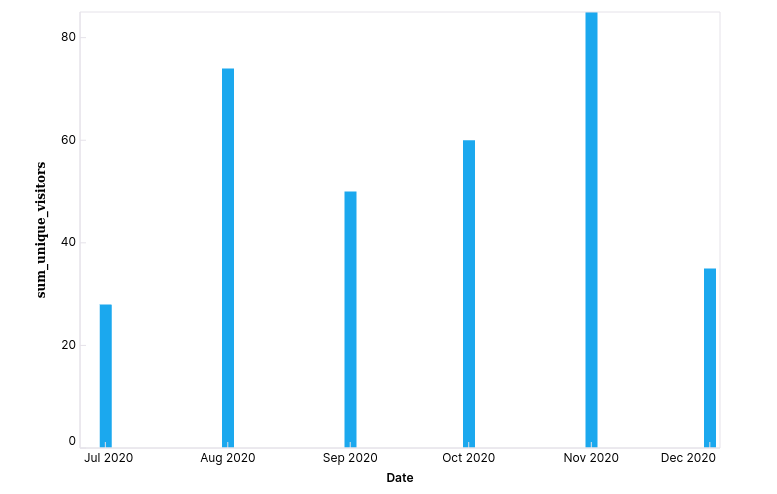
\includegraphics[width=\linewidth]{images/access-overall.png}
\label{fig:accessOverall}
\end{figure}

Looking at the number of unique visitors, we can see a spike in August, most likely for the coverage of the preparation for the latest global climate strike and in November, when the second lockdown started. I would assume that December's figures are probably a bit too low as I have collected the data before the end of the month.

\subsection{Access by Country}

Where do all the visitors of the blog come from? Let's first have a look at the distribution by country:

\begin{figure}[H]
\centering
\caption {Access by Country}
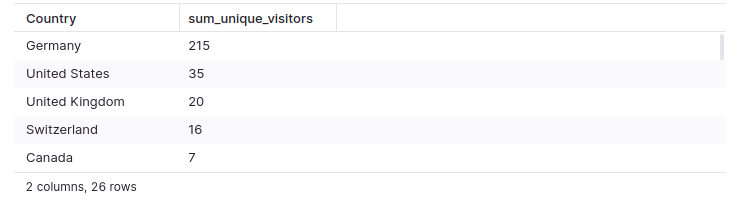
\includegraphics[width=\linewidth]{images/access-country.png}
\label{fig:accessCountry}
\end{figure}

Not surprisingly, most visitors access the blog from Germany, my home country, immediately followed by the United States and the United Kingdom. I write the blog in English so that visitor distribution makes total sense. Looking at the access number from the German-speaking countries alone, I might get a higher number of visitors if the blog was in German. Still, I would lose all visitors from countries other than Germany, Austria, and Switzerland. For now, I will keep writing blog posts in English.

\subsection{Access by Operating System}

The blog's visitors not only originate from countries, but also from operating systems:

\begin{figure}[H]
\centering
\caption {Access by Operating System}
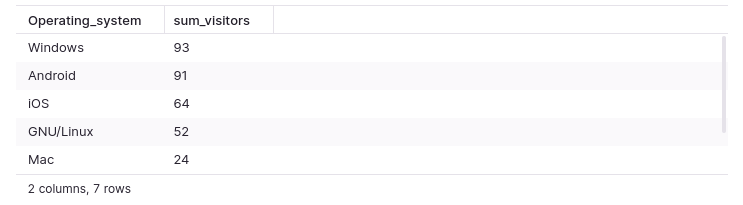
\includegraphics[width=\linewidth]{images/access-os.png}
\label{fig:accessOS}
\end{figure}

and browsers:

\begin{figure}[H]
\centering
\caption {Access by Browser}
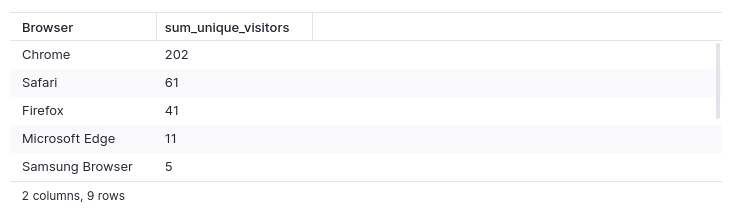
\includegraphics[width=\linewidth]{images/access-browser.png}
\label{fig:accessBrowser}
\end{figure}

Chrome is still the undisputed market leader in browsing, and I know that the WordPress theme in use for the blog displays well on Chrome. 

Looking at the operating system, we can deduct that there is about equal access from mobile devices (Android + iOS) and Desktop devices (Windows + Linux + Mac). I will need to make sure that the WordPress theme I use is well suited for mobile devices.

\subsection{Access by Referral}

In addition to the number of visitors, there are other interesting KPIs, especially visit duration and bounce rate. Let's look at these KPIs first by referral:

\begin{figure}[H]
\centering
\caption {Access by Referral}
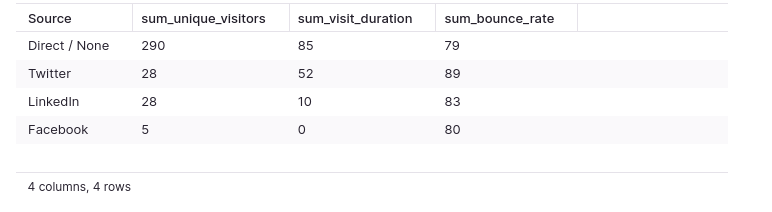
\includegraphics[width=\linewidth]{images/access-referral.png}
\label{fig:accessReferral}
\end{figure}

We can see that direct access to the blog has the highest number of unique visitors, the most prolonged visit duration, and the lowest bounce rate. This is not surprising; people who actively seek out the blog most likely have the highest interest in its content.

My cross-posts to Twitter, LinkedIn, and Facebook yield a lot fewer visits, with Facebook being the outlier, generating almost no visitors and no visit duration. In the future, I might review cross-posting to Facebook and stop the practice if the numbers do not improve. 

I did not expect the cross-posts to LinkedIn to yield any visits and am pleasantly surprised; without looking at the data, I would have assumed that access from Facebook would be much higher than from LinkedIn.

\subsection{Access by Source}

Second, let's look at these KPIs by source:

\begin{figure}[H]
\centering
\caption {Access by Source}
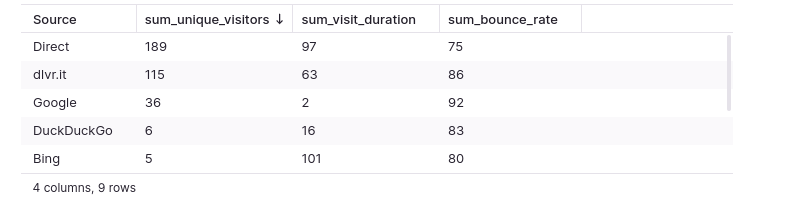
\includegraphics[width=\linewidth]{images/access-source.png}
\label{fig:accessSource}
\end{figure}

As expected, we can see the same picture here, direct access to the blog has the highest number of unique visitors, the most prolonged visit duration, and the lowest bounce rate.

However, access from the search engines is a lot less than from cross-posting through dlvr.it, which I did not expect. To improve this, I might need to review the Google Search Console settings and pay closer attention to tags and keywords.

Just by looking at the data, I was already able to gain some insights into the visitors' behavior and identify some possible improvements for the future.

\subsection{Categories}

As a next data point, we'll want to look at the content of the blog posts. First, we'll have a look at the list of categories taken from the blog:

\begin{itemize}
\item buddhism
\item climateaction
\item climateemergency
\item climatestrike
\item cloudnative
\item electric-cars
\item fridaysforfuture
\item kubernetes
\item leavenoonebehind
\item movies
\item music
\item politics
\item rancher
\item socialmedia
\item travel
\item university
\item youtube
\end{itemize}

I have omitted two, cologne and general, from the blog's categories, as they are present on all posts. These categories are at the same time hashtags for Diaspora*, another social network that I cross-post to; Diaspora* is part of the Fediverse and does not have the same reach as the more popular commercial networks and thus did not appear in the statistics above. Interactions on Diaspora* are far fewer than on the other networks, but they tend to be more thoughtful and exciting.

To prepare for the analysis, I have decided to reduce the number of categories down to four, based on the distribution of the posts in the WordPress dashboard:

\begin{itemize}
\item Climate and politics (1)
\item Cloud (2)
\item Social Media and culture (3)
\item Covid-19 (4)
\end{itemize}

Climate and politics will include all posts regarding our major crisis, the climate emergency, and the climate justice movement.

Cloud will include all posts in regards to cloud-native technology.

Social Media and culture will include posts on YouTube, music, and movies.

Covid-19 will cover all posts related to the other crisis, the current global pandemic.

 If there's a blog post without a category, I will encode the missing value with 0.

These four content categories should help us in the next chapter analyzing the individual blog post performance and possibly arrive at more insights and finally, at some predictions.

\subsection{Blog Post Sentiment}

The final data point to explore is the sentiment of the post.

From the many available libraries for Python I've chosen VADER (Valence Aware Dictionary and sEntiment Reasoner) based on the description of the algorithm and its results in an analysis and ranking of texts by H.P. Lovecraft.\footnote{See \textit{Pocs, M. (2018)}: Lovecraft with Natural Language Processing.\cite{lovecraftAnalysis}}

Vader is "specifically attuned to analyzing social media posts"\footnote{\textit{Hutto, C. (2018)}: VADER Sentiment Analysis.\cite{vaderReadme}} and thus the perfect choice to analyze blog posts; Vader can also be used just with a few lines of code, making it an ideal library for casual analysis such as this one. 

With an extensive data set, there would have been the option to create and train a more specific NLP machine learning model to identify the post's sentiment. For a small data set like the blog, I felt it would be more prudent to use a ready-made library.

Let's look at an example invocation:

\begin{lstlisting}[caption=Vader Example, frame=single, basicstyle=\ttfamily]
from vaderSentiment.vaderSentiment 
  import SentimentIntensityAnalyzer

blogPost = "My first ever entirely virtual Christmas and 
  it went quite well! And so will New Years, I hope."

analyzer = SentimentIntensityAnalyzer()

print(analyzer.polarity_scores(blogPost))

\end{lstlisting}

The text in the example is the first sentence of the most recent post and Vader will show the following sentiment rating:

\verb|{'neu': 0.74, 'compound': 0.68, 'neg': 0.0, 'pos': 0.26}|

We know that compound is the normalized, weighted composite score of the other three values (positive, negative, and neutral) from the documentation. I'll be using the sentiment compound values to enrich our data.\footnote{See \textit{Hutto, C. (2018)}: VADER Sentiment Analysis.\cite{vaderReadme}} The compound will have values between 1 (most positive) and -1 (most negative), and there won't be any missing values; a value of 0 will indicate a completely neutral text.

\subsection{Data Source}

For the data analysis and visualization in this chapter, I used a Count data notebook; you can find the raw data and all charts from this chapter here: \href{https://count.co/n/6WKuBzDV4Qq}{WTA Chapter 3}


%
%	Praxisbezug
%

\pagebreak
\section{Data Analysis}

\onehalfspacing

\subsection{Correlation between blog post categories and performance}

Text 

\subsection{Correlation between blog post sentiment and performance}

Text

\subsection{Predictions}

Text


%
%	Fazit
%

\pagebreak
\section{Summary}

\onehalfspacing

Text

You can find all data sources on   \href{https://github.com/chfrank-cgn/Rancher/tree/master/az-cluster-1}{GitHub}.

Happy Analysis!


% Literaturverzeichnis
\cleardoublepage
\raggedright
\bibliographystyle{IEEEtranS}	% ieeetran verwenden, damit auch URLs angezeigt werden
\bibliography{seminar-lit}

\cleardoublepage
\justify
%
%	Ehrenwoertliche Erklaerung
%

\pagebreak

\pagenumbering{gobble} % Keine Seitenzahlen mehr
\onehalfspacing

%-----------------------------------
% Ehrenwoertliche Erklärung
%-----------------------------------
\section*{Declaration in lieu of oath}

\par\medskip

I, with this, declare that I produced the submitted paper with no assistance from any other party and without the use of any unauthorized aids and, in particular, that I have marked as quotations all passages which are reproduced verbatim or near-verbatim from publications. Also, I declare that the submitted print version of this thesis is identical to its digital version. Further, I say that this thesis has never been introduced to any examination board in either its present form or in any other similar version. I herewith agree that this thesis may be published. I herewith consent that this thesis may be uploaded to the server of external contractors to submit it to the contractors’ plagiarism detection systems. Uploading this thesis to send it to plagiarism detection systems is not a form of publication.

\par\medskip
\par\medskip

\vspace{5cm}

\begin{table}[H]
	\begin{tabular*}{\textwidth}{c @{\extracolsep{\fill}} ccccc}
		Cologne, \the\month/\the\day/\the\year \\
		\rule[0.5ex]{12em}{0.55pt} & \rule[0.5ex]{12em}{0.55pt} \\
		(Location, Date) & (Signature)
	\end{tabular*}
\end{table}


\end{document}
